\graphicspath{{sec02/images/}}
\lstset{inputpath=sec02/code}
% \setminted{inputpath=sec02/code/}



%%%%%%%%%%%%%% WYSiWYG %%%%%%%%%%%%%%%%%%%%%%
\begin{frame}{WYSiWYG vs not-WYSiWYG approaches}
\begin{columns}[c]
        \begin{column}{0.45\textwidth}
{\csk WYSiWYG} -- \textit{What You See is What You Get} approach\\~\\



\inclassFrag{Examples?}[1]
\end{column}
\inpause
\begin{column}{0.45\textwidth}
Microsoft Word
\begin{center}
        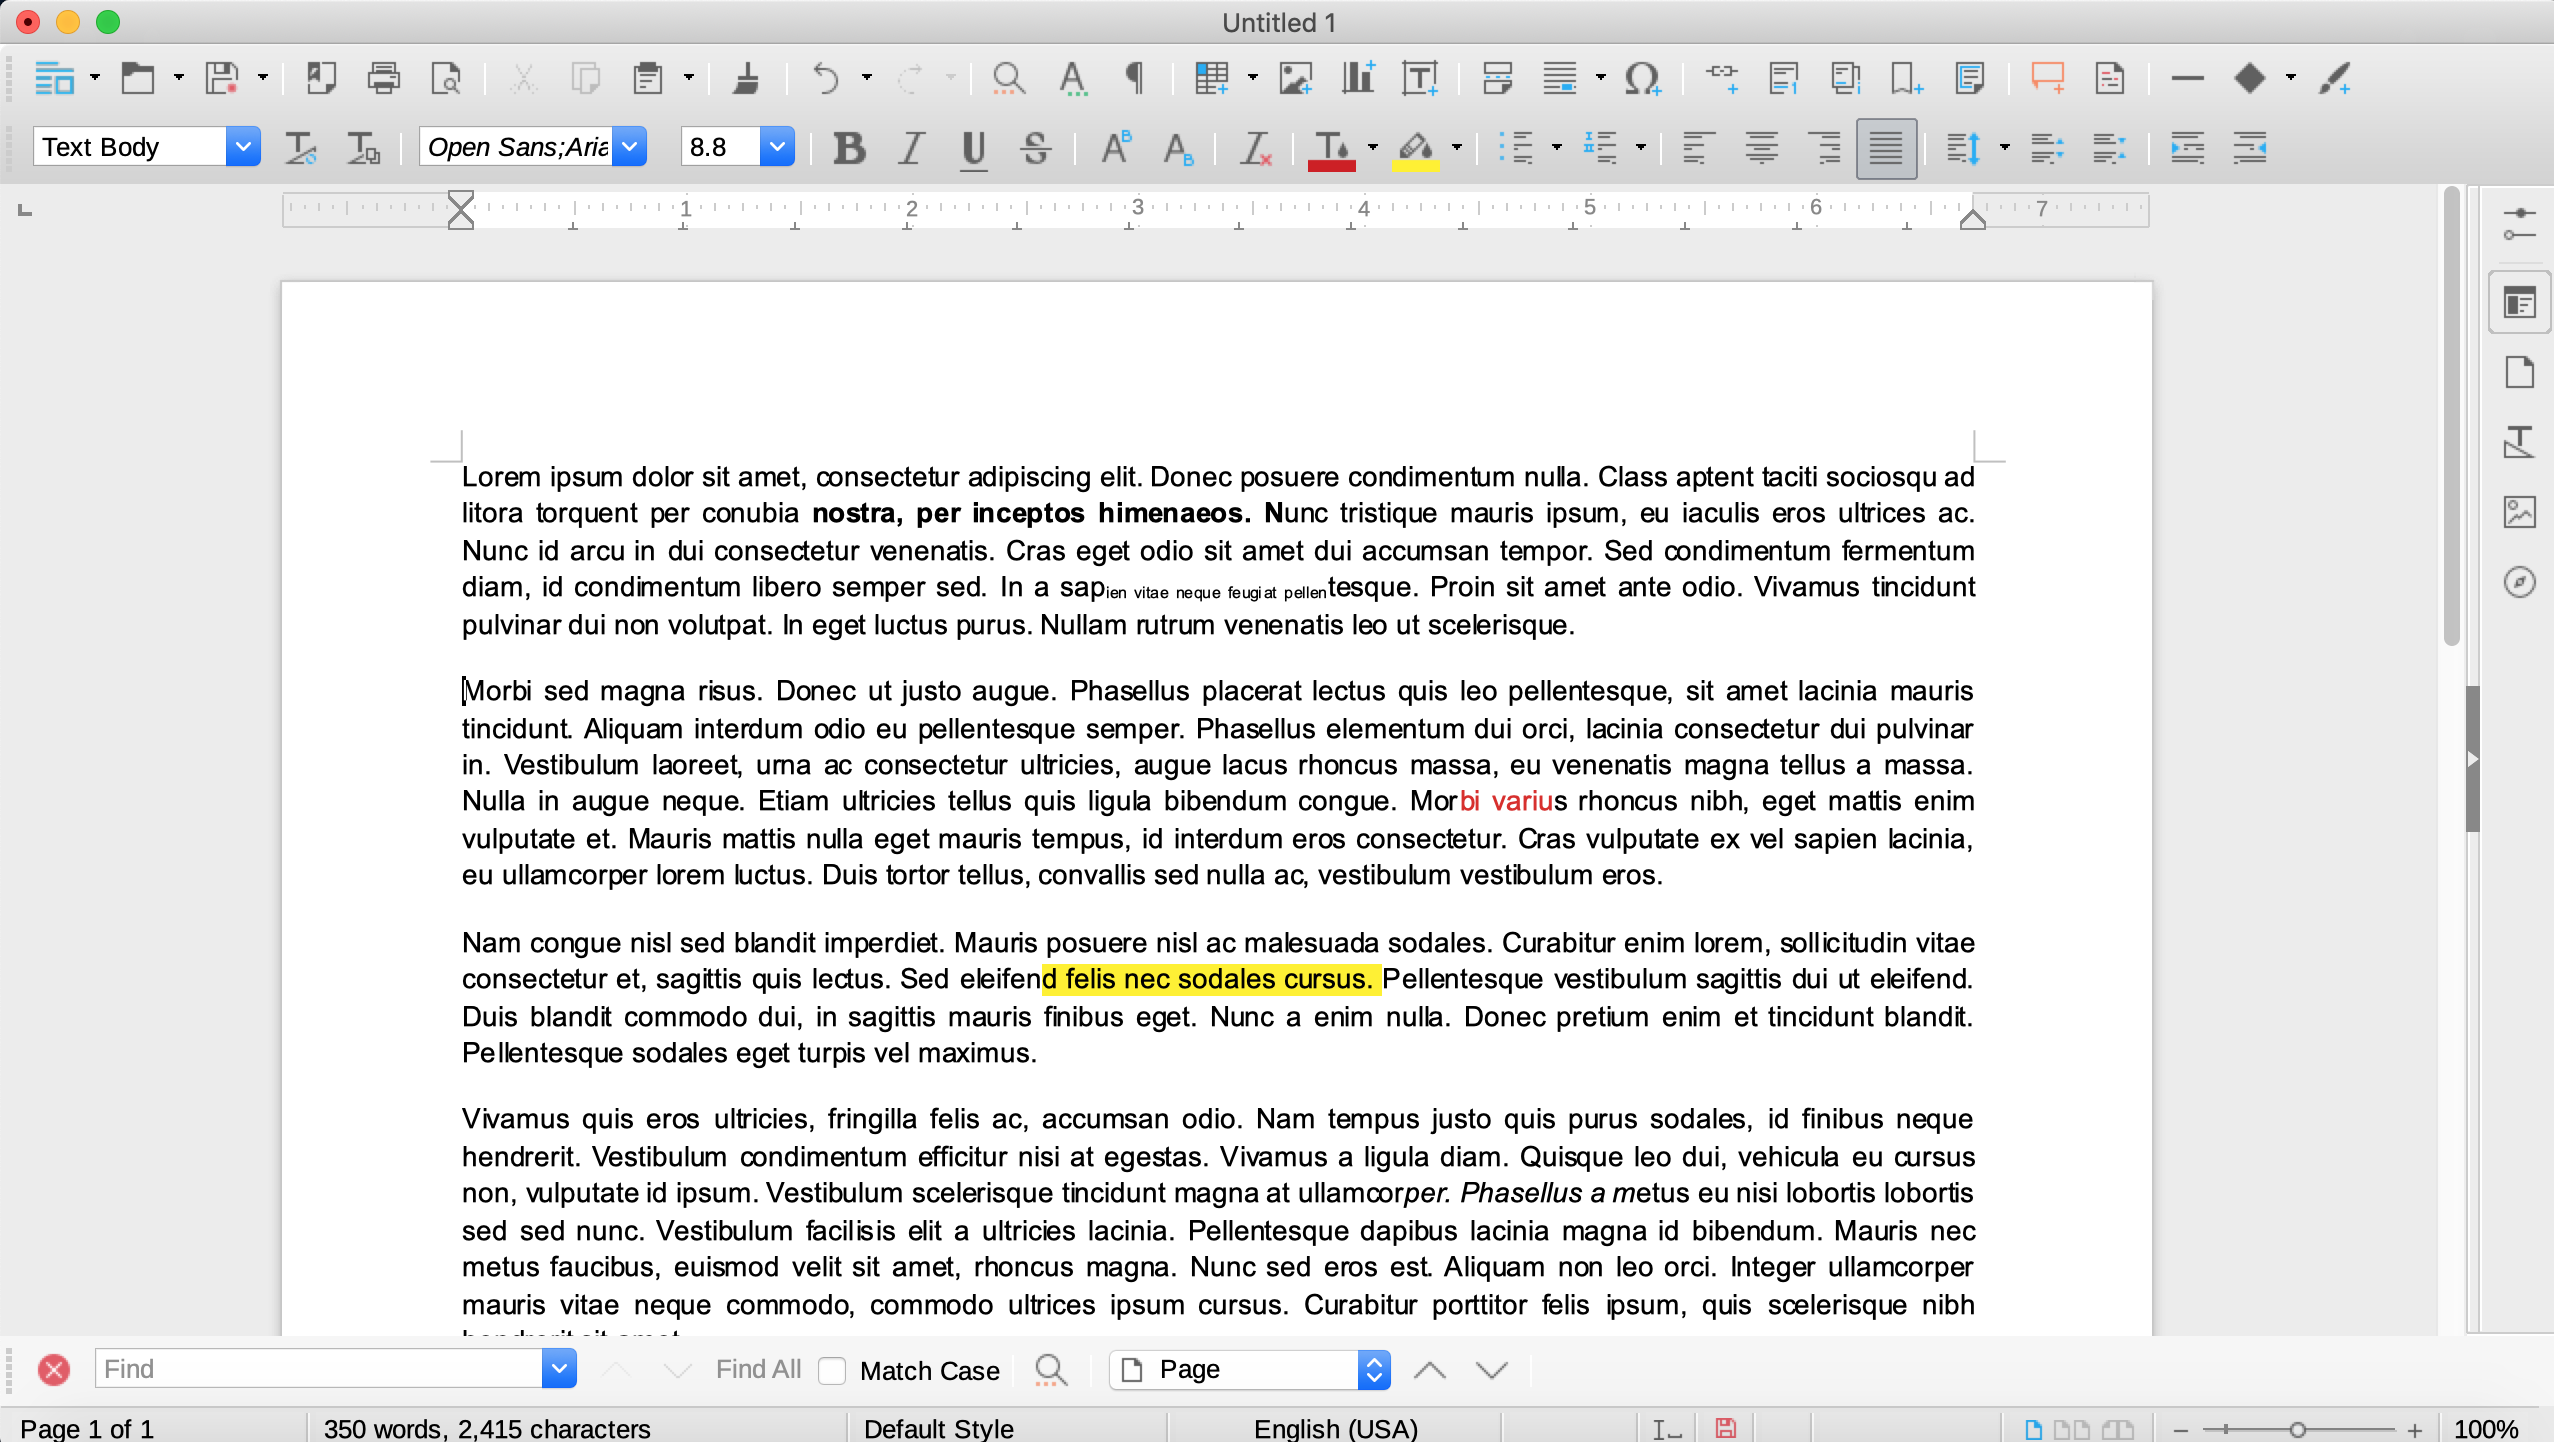
\includegraphics[width=\textwidth,height=0.6\textheight,keepaspectratio]{wysiwyg.png}%
    \end{center}
        \end{column}
    \end{columns}
\end{frame}

\begin{frame}[fragile]{not-WYSiWYG}\relax
\skfootnote{about \TeX\ and CSS \normalfont \url{https://www.wiumlie.no/2006/phd/}}
\inclassFrag{Examples?}[1]
HTML and CSS 
\cprotect\twocolImg{
\begin{minted}{html}
<html>
  <head>
    <meta charset="utf-8">
  </head>
  <style>h1{color:red;}</style>
  <body>
    <h1>Header</h1>
    <i>Hello</i>,<br/> world!  <!-- comment -->
  </body>
</html>
\end{minted}
}{HTML1}
\inpause

\cprotect\twocolImg{
\begin{minted}{html}
...
  <style>h1{color:green;}</style>
...
\end{minted}
}{HTML2}

\inpause
{\csk CSS} was most probable created influenced by \TeX
\end{frame}


\begin{frame}[fragile]{not-WYSiWYG}\relax

\LaTeX
\cprotect\twocolImg{
\inputminted{latex}{sec02/code/helloworld.tex}
}{LaTeX1}
\inpause

\cprotect\twocolImg{
\begin{minted}{latex}
...
  \titleformat*{\section}{\LARGE\bfseries\color{green}}
...
\end{minted}
}{LaTeX2}

\end{frame}

\begin{frame}[fragile]{Compare HTML and \LaTeX }\relax
    \begin{columns}
        \begin{column}{0.5\textwidth}
\begin{minted}{html}
<html>
  <head>
    <meta charset="utf-8">
  </head>
  <style>h1{color:red;}</style>
  <body>
    <h1>Header</h1>
    <i>Hello</i>,<br/> world!  <!-- comment -->
  </body>
</html>
...
  <style>h1{color:green;}</style>
...
\end{minted}
\end{column}
        \begin{column}{0.5\textwidth}
\inputminted{latex}{sec02/code/helloworld.tex}
\begin{minted}{latex}
...
  \titleformat*{\section}{\LARGE\bfseries\color{green}}
...
\end{minted}
\end{column}
    \end{columns}
\end{frame}

\cprotect\inclassframe{
\begin{frame}[fragile]{\exFrame{Try to compile your first doc}}\relax
    \inputminted[fontsize=\normalsize]{latex}{sec02/code/first.tex}
    %  \lstinputlisting[basicstyle=\tt\small, numbers=none]{first.tex}
\end{frame}
}
\begin{frame}[fragile]{Document structure}{overview}
\inputminted{latex}{sec02/code/structureOfDocument.tex}
    % \lstinputlisting{structureOfDocument.tex}
    
    \skfootnote{\lvoc{I.2.4}[20] \wikiC{https://en.wikibooks.org/wiki/LaTeX/Basics\#Our_first_document} \overC{https://www.overleaf.com/learn/latex/Creating_a_document_in_LaTeX}}
\end{frame}

\begin{frame}[fragile]{Document structure}{class files}

Class of the document is responsible for the large-scale settings
    \cprotect\skfootnote{\lvoc{IV.1}, \lamc{2.2.2} \url{https://texblog.org/2013/02/13/latex-documentclass-options-illustrated/}\\ environment \lstinline|tabbing|} 
{
\scriptsize
\begin{tabbing}
\lstinline|\documentclass|\hspace{-1ex} \= \lstinline|[10pt,|  \= \lstinline|onecolumn,|  \=  \lstinline|a4paper]|\hspace{-1ex} \= \lstinline|{article}| \kill
\> \> \> \> \lstinline|{beamer} %presentation, poster| \\
\> \> \> \> \lstinline|{report}| \\
\> \> \> \> \lstinline|{book}| \\
\> \> \> \> \lstinline|{standalone} %for one picture/equation| \\
\> \> \> \> \lstinline|{extarticle} %if you want 14pt font size| \\
\lstinline|\documentclass| \> \lstinline|[10pt,|  \> \lstinline|onecolumn,|  \>  \lstinline|a4paper]| \> \lstinline|{article}| \\ 
\> \lstinline|[12pt] %fontsize| \> \\ 
\> \> \lstinline|[twocolumns] %number of columns in document| \> \\ 
\> \> \> \lstinline|[a5paper] %paper size| \> \\ 
\end{tabbing}}
\cprotect\skfootnote{\lmanc{3}[17]\\ in this presentation \verb|[aspectratio=169]|}
\end{frame}
\note{
but there is no ``fixed set'' of classes. Can build our own 
}

%%TSK: предложить создать документ и поиграться с параметрами
\begin{frame}[fragile]{Document structure}{style files}
     Style files are responsible for settings and providing new commands 
     
     \vfill
     \hspace{-1ex}
     \lstinline[basicstyle=\tt\large]|\usepackage[optional]{necessary}{packagename}|
     \vfill
\end{frame}

\cprotect\inclassframe{
\begin{frame}[fragile]{\exFrame{Try to add the following before begin document}}

\begin{minted}{latex}
    \usepackage{geometry}
    \geometry{paperwidth=80mm, paperheight=50mm, left=5mm, top=5mm, right=5mm, bottom=5mm}
\end{minted}
\end{frame}
}

\note{practicully everything is from package }
% сначала тут скомпилировать док. Потом добавить туда какую-то команду с параметром. Потом показать уже общую схему

\begin{frame}[fragile]{Commands}
    \lstinline[basicstyle=\tt\large]|\command[o1, o2]{n1, n2=value}[o3]{n3}|\par
    (o = optional argument, n = necessary argument)~\\[2ex]

\pause
    \skfootnote{\knuthc{3}[19], \lvoc{I.2.3}[19], \lvoc{I.2.7}[24], \wikiC{https://en.wikibooks.org/wiki/LaTeX/Basics}
    }

    {\csk Command symbols}
    \verb|\$ \# \{ \} \^{} \& \_ \~{} \\|
    \vfil
    {\csk Command words}
    \verb|\sin \LaTeX \Rightarrow \qquad|
    
    {\csk Environments}
    \verb|\begin{frame}\end{frame}  \begin{equation}\end{equation}|
    
\end{frame}